\documentclass[12pt, a4paper]{article}
\usepackage{amsmath}
\usepackage{amsfonts}
\usepackage{amsthm}
\usepackage{mathtools}
\newtheorem{theorem}{Theorem}[section]
\newtheorem{definition}{Definition}[section]
\numberwithin{equation}{section}
\usepackage{pgfplots}
\pgfplotsset{width=10cm,compat=1.9}
\graphicspath{ {img/} }
\DeclareGraphicsExtensions{.png}

\title{Softmax function}
\author{Kristian Wichmann}

\begin{document}
\maketitle

\section{Definition}
Given an $n$-dimensional input vector $z$, the \textit{softmax function} (also known as the \textit{normalized exponential function}), has the output:
\begin{equation}
\sigma_i(z)=\frac{e^{z_i}}{\sum_{k=1}^n e^{z_k}}
\end{equation}
This means, that the outputs can be interpreted as an discrete probability distribution, since they will always sum to 1.

It will be convenient to give a shorthand for the normalization "constant", so we set:
\begin{equation}
N(z)=\sum_{k=1}^n e^{z_k}
\end{equation}

\subsection{Example}
Figure \ref{fig:softmax_example} shows the softmax function applied to the set $\{1, 2, 3,\cdots, 8\}$. As is evident, comparatively small values are given much less overall weight than higher ones.

\begin{figure}
\centering
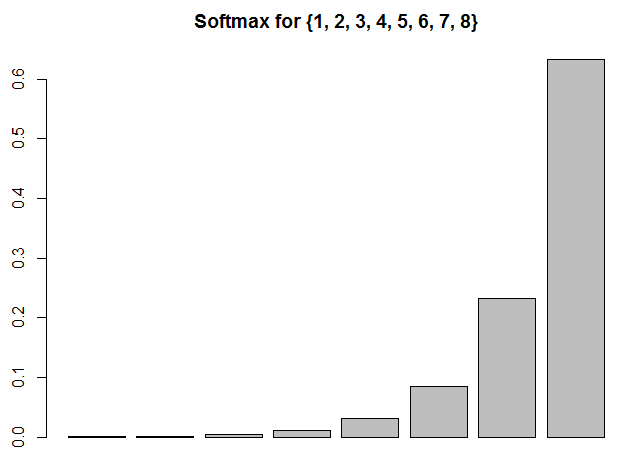
\includegraphics[width=0.75\textwidth]{softmax_example}
\caption{Softmax example}
\label{fig:softmax_example}
\end{figure}

\section{Derivative}
We might now want to differentiate with respect to the component $z_j$, which is done by applying the quotient rule:
\begin{equation}
\label{quotient}
\frac{\partial\sigma_i(z)}{\partial z_j}=\frac{\partial}{\partial z_j}\frac{e^{z_i}}{N(z)}=\frac{\left(\frac{\partial}{\partial z_j}e^{z_i}\right)N(z)-e^{z_i}\left(\frac{\partial}{\partial z_j}N(z)\right)}{(N(z))^2}
\end{equation}
The two derivatives are:
\begin{equation}
\frac{\partial}{\partial z_j}e^{z_i}=\delta_{ij}e^{z_i},\quad\frac{\partial}{\partial z_j}N(z)=\sum_{k=1}^n\delta_{jk}e^{z_k}=e^{z_j}
\end{equation}
Inserting into equation \ref{quotient} this yields:
\begin{equation}
\frac{\delta_{ij}e^{z_j}N(z)-e^{z_i+z_j}}{(N(z))^2}
\end{equation}
The numerator can be rewritten:
\begin{equation}
e^{z_i}\left(\delta_{ij}N(z)-e^{z_j}\right)
\end{equation}
Now divide by $N(z)$ twice, once "outside the parenthesis" and once "inside" to get:
\begin{equation}
\label{derivative}
\frac{\partial\sigma_i(z)}{\partial z_j}=\frac{e^{z_i}}{N(z)}\left(\delta_{ij}-\frac{e^{z_j}}{N(z)}\right)=\sigma_i(z)\left(\delta_{ij}-\sigma_j(z)\right)
\end{equation}
The likeness to the derivative of the logistic function should be evident.

\section{Cross-entropy error function}
The softmax is often combined with a cross-entropy error function for classification:
\begin{equation}
J(z)=\sum_{i=1}^n t_i\log\sigma_i(z)=\sum_{i=1}^n t_i\log y_i
\end{equation}
Here $t_i$ represents the label for the data and $y_i=\sigma_i(z)$ is the softmax output. For classification, this is simply $t_i=\delta_{ic}$, where $c$ is the correct label. In this case, the error function is simply:
\begin{equation}
J(z)=\sum_{i=1}^n\delta_{ic}\log\sigma_i(z)=\log\sigma_c(z)=y_c
\end{equation}
The derivative with respect to $z_i$ is found through the chain rule:
\begin{equation}
\frac{\partial J}{\partial z_i}=\frac{\partial J}{\partial y_c}\frac{\partial y_c}{\partial z_i}=\frac{\partial}{\partial z_i}\log\sigma_c(z)\frac{\partial\sigma_c}{\partial z_i}=\frac{1}{\sigma_c(z)}\sigma_c(z)\left(\delta_{ci}-\sigma_i(z)\right)=\delta_{ic}-y_i
\end{equation}
But this is exactly the difference between the real value $t_i$ and the output $y_i$, also known as the \textit{error} $\delta_i=t_i-y_i$:
\begin{equation}
\frac{\partial J}{\partial z_i}=\delta_i
\end{equation}

\end{document}